% Master's qualification text (EPUSP / PPGEE). Self-contained folder for Overleaf:
% upload or sync the whole quali/ directory; main document = main.tex; compiler = pdfLaTeX; bibliography = BibTeX.
\documentclass[]{politex-xico}

% ========== Packages ==========
\usepackage[utf8]{inputenc}
\usepackage{amsmath,amsthm,amsfonts,amssymb,mathtools}
\usepackage{graphicx,enumerate}
\usepackage{multirow}
\usepackage{booktabs,tabularx}
\usepackage[normalem]{ulem}
\usepackage[alf,abnt-etal-list=0]{abntex2cite-xico}
\usepackage[english]{babel}
\usepackage[table]{xcolor}
\usepackage{todonotes}
\usepackage{tikz}
\usetikzlibrary{positioning,arrows.meta}
\DeclareMathOperator*{\argmax}{arg\,max}
\newcommand{\recallk}[1]{\mathrm{R@}#1}

% ========== Document data ==========
\titulo{Chain-Following as a Low-Rank Skill: Cheap Evidence Selection for Multi-Hop Retrieval-Augmented Generation}
\autor{ARNOLD ALVARO MOYA LAVADO}
\orientador{Prof. Dr. Anna Helena Reali Costa}
\qualificacaoMestrado{Electrical Engineering}
\departamento{Computação e Sistemas Digitais - PCS}
\areaConcentracao{Computer Engineering}
\local{São Paulo}
\data{2026}

\begin{document}
\capa
\falsafolhaderosto
\folhaderosto

% ========== Abstract ==========
\begin{abstract}
Retrieval-augmented generation (RAG) lets a large language model (LLM) answer from external evidence, but every retrieved paragraph sent to the LLM costs tokens, and distractors can lower answer quality. For multi-hop questions the problem is harder, because later evidence is often only weakly related to the question itself. This work studies \emph{cheap evidence selection}: a small cross-encoder (22.7M parameters) decides which paragraphs the LLM sees.

Preliminary results support three findings. First, a fine-tuned small selector sends 68--77\% fewer prompt tokens than sending the ten retrieved paragraphs, at statistically indistinguishable answer F1 on HotpotQA; adaptive stopping saves further tokens on HotpotQA and MuSiQue. Second, on MuSiQue the one-shot ranker is the bottleneck, and re-scoring with the question plus the paragraphs already selected (iterative reranking) appeared to help. A pair-matched control, however, showed that part of that gain came from additional training data. Third, the ability to use such a conditioned query is a \emph{separable, low-rank} change: a rank-2 approximation of the weight difference recovers about 85\% of its effect, against 7--9\% for norm-matched random controls, and it helps long chains. On 566 fresh four-hop questions, conditioning-trained iteration improves full-support recall@5 by 0.055 (95\% CI $[0.007, 0.102]$), while a router that predicts hop count does not yield a useful cascade.

All experiments were pre-registered in a version-controlled repository, with paired statistical tests and an explicit record of null results. The remaining work turns the findings into a reusable artifact: a rank-2 \emph{chain adapter} trained directly as a low-rank update, a router that decides when to activate it, a transfer test across rerankers and datasets, and an evaluation of answer quality.

\textbf{Keywords:} retrieval-augmented generation, multi-hop question answering, evidence selection, cross-encoder reranking, low-rank adaptation.
\end{abstract}


\tableofcontents

\chapter{Introduction}
\label{chap:intro}

\section{Context}

Large language models store knowledge in their parameters, but this \emph{parametric} knowledge is hard to update, hard to attribute and prone to errors \cite{pmlr-v119-guu20a,3495724.3496517,liu2026unifieddefinitionhallucinationits}. Retrieval-augmented generation (RAG) adds a \emph{non-parametric} memory: a retriever finds passages, and the LLM conditions its answer on them \cite{3495724.3496517,pmlr-v119-guu20a}. This makes answers easier to update and to verify, but it moves part of the cost to the prompt. Every passage sent to the LLM is paid for in input tokens, and passages that do not support the answer can mislead the model \cite{liu2024lostinthemiddle,wang2023filco}.

Multi-hop questions make this trade-off sharper. In a question such as ``In which city was the founder of the company that makes product $X$ born?'', the second and third pieces of evidence share little vocabulary with the question; they are related to the evidence found in the previous step \cite{yang2018hotpotqa,trivedi2022musique}. A selector that scores each passage against the question alone tends to rank such \emph{bridge} passages low, so a system either sends many passages, which is expensive, or risks losing the chain.

\section{Problem and research questions}

This work studies \emph{cheap evidence selection} for multi-hop RAG: a small model, much cheaper than the LLM, decides which retrieved paragraphs the LLM sees. The cost of interest is the LLM's input tokens, plus the selector's own compute, measured as cross-encoder forward passes. The questions are:

\begin{description}
  \item[RQ1] How many prompt tokens can a small fine-tuned cross-encoder save at equal evidence recall and answer quality?
  \item[RQ2] On harder multi-hop data, is the limit the stopping rule (how many passages to send) or the ranker itself?
  \item[RQ3] Does conditioning the ranker on the passages already selected (iterative reranking) help, once confounds such as the amount of training data are controlled?
  \item[RQ4] What is the structure of the weight change that gives a small reranker this chain-following ability, and can it be isolated as a small, reusable component?
\end{description}

\section{Hypothesis}

The central hypothesis is that \textbf{chain-following in a small reranker is a separable, low-rank skill that matters mainly for long reasoning chains}. If it holds, the skill can be shipped as a small adapter on top of a cheap one-shot selector and switched on only where it helps, keeping short questions cheap.

\section{Contributions so far}

\begin{enumerate}
  \item An evaluation of a 22.7M-parameter cross-encoder as an evidence selector, with token accounting at matched recall and answer F1 (HotpotQA, MuSiQue).
  \item Evidence that, on MuSiQue, the one-shot ranker rather than the stopping rule limits cost, and a pair-matched control showing that part of the apparent benefit of iterative reranking came from additional training data.
  \item Evidence that the ability to use a conditioned query is a rank-2 weight change (about 85\% of its effect recovered, random controls 7--9\%), and a pre-registered confirmation that it helps four-hop chains.
  \item A research protocol for an AI-assisted project: pre-registration of every decision rule in version control, paired statistics, adversarial review of each protocol before running it, and a claim ledger that records null results (Section~\ref{sec:protocol}).
\end{enumerate}

\section{Organization}

Chapter~\ref{chap:background} introduces RAG, multi-hop question answering, cross-encoder reranking and the structure of fine-tuning updates. Chapter~\ref{chap:related} positions this work against related research. Chapter~\ref{chap:method} describes the models, data, inference procedures, analyses and the research protocol. Chapter~\ref{chap:results} reports the preliminary results. Chapter~\ref{chap:plan} presents the remaining work, the planned artifact and the schedule. Appendix~\ref{app:index} lists every experiment run so far, including those not used in this text.

\chapter{Background}
\label{chap:background}

This chapter introduces the concepts the rest of the text relies on: retrieval-augmented generation, multi-hop question answering, cross-encoder reranking, the structure of fine-tuning updates, and the evaluation metrics and statistical tests used.

\section{Parametric and non-parametric knowledge}

A Transformer language model \cite{vaswani2017attention} stores what it learned in its weights. This \emph{parametric} knowledge is implicit: it cannot be inspected or updated piece by piece, and the model may produce fluent but unsupported statements. \citeonline{liu2026unifieddefinitionhallucinationits} define such hallucinations as failures of the model's internal world model and propose a taxonomy of errors. Recent post-training methods improve reasoning, for example reinforcement learning with verifiable rewards \cite{Guo_2025,lambert2025tulu3pushingfrontiers}, but they do not remove the need for up-to-date, attributable evidence.

Retrieval-augmented models add a \emph{non-parametric} memory. REALM \cite{pmlr-v119-guu20a} trains a retriever jointly with a masked language model; RAG \cite{3495724.3496517} conditions a generator on passages from a dense retriever. In the systems studied here the LLM is used as a fixed reader: a retriever returns candidate paragraphs, a selector chooses some of them, and the LLM answers from the selected ones.

\section{Multi-hop question answering}

A question is \emph{multi-hop} when its answer requires combining several pieces of evidence. HotpotQA \cite{yang2018hotpotqa} provides two-hop questions with ten candidate paragraphs each, two of them supporting and eight distractors. MuSiQue \cite{trivedi2022musique} composes two- to four-hop questions from single-hop ones and filters out questions that can be answered by shortcuts; each question has about twenty candidate paragraphs. In both datasets the supporting paragraphs are annotated, so evidence recall can be measured without an LLM. 2WikiMultiHopQA \cite{ho2020twowiki} is a third, related benchmark planned for the remaining work.

\section{Cross-encoder reranking}

A \emph{bi-encoder} embeds the question and each paragraph separately and compares the embeddings, which is fast but loses interactions between them \cite{reimers2019sentence}. A \emph{cross-encoder} reads the question and the paragraph together and outputs a single relevance score \cite{nogueira2019passage}. It is more accurate but needs one forward pass per (question, paragraph) pair. This work uses \texttt{ms-marco-MiniLM-L6-v2}, a six-layer MiniLM \cite{wang2020minilm} cross-encoder with 22.7M parameters trained for passage reranking on MS MARCO \cite{bajaj2016msmarco}. Scoring the twenty paragraphs of a MuSiQue question takes twenty forward passes.

\textbf{One-shot and iterative reranking.} A one-shot reranker scores every paragraph against the question once and sorts them. An \emph{iterative} reranker selects one paragraph at a time and re-scores the remaining ones with a query that contains the question and the paragraphs already selected. Iterative selection can follow a chain from one piece of evidence to the next, at the cost of more passes \cite{xiong2021mdr,zhang2024beamretrieval}.

\section{Structure of fine-tuning updates}

Fine-tuning changes a pretrained weight matrix $W_0 \in \mathbb{R}^{m \times n}$ into $W_1 = W_0 + \Delta$. Several lines of work show that useful updates are often well approximated in a low-dimensional subspace. \citeonline{aghajanyan2021intrinsic} measure a low intrinsic dimension of fine-tuning, and LoRA \cite{hu2022lora} trains only a low-rank update $\Delta = BA$ with $B \in \mathbb{R}^{m \times r}$, $A \in \mathbb{R}^{r \times n}$ and small $r$. Given a full update, its best rank-$r$ approximation in the Frobenius norm is the truncated singular value decomposition,
\begin{equation}
\Delta_r = \sum_{i=1}^{r} \sigma_i u_i v_i^\top,
\label{eq:svd}
\end{equation}
where $\sigma_1 \ge \sigma_2 \ge \dots$ are the singular values of $\Delta$ and $u_i, v_i$ the corresponding singular vectors \cite{vasani2025phlora}. Task vectors, the differences between fine-tuned and base weights, can also be added or subtracted to transfer behaviour between models \cite{ilharco2023taskarithmetic,yadav2023ties}.

\section{Metrics}

\begin{description}
  \item[Full-support recall@$k$.] The fraction of questions whose top-$k$ selected paragraphs contain \emph{all} supporting paragraphs. A question with three supporting paragraphs counts only if all three are selected. This is stricter than the usual per-paragraph recall, and matches what a reader needs to answer a multi-hop question.
  \item[Tokens.] The number of input tokens of the reader's prompt with the selected paragraphs, counted with the reader's tokenizer (\texttt{o200k\_base}) or as reported by the API.
  \item[Passes.] Cross-encoder forward passes per question, the selector's compute cost.
  \item[Answer F1 and EM.] Token-level F1 and exact match between the reader's answer and the reference answer (maximum over aliases), after standard normalization.
\end{description}

\section{Statistical tests}

All comparisons are paired: two systems are evaluated on the same questions. For binary per-question outcomes (for example, whether all supporting paragraphs are in the top five), the exact McNemar test uses only the discordant questions \cite{mcnemar1947}. For differences in means (tokens, F1), 95\% confidence intervals are obtained with the paired bootstrap over questions \cite{efron1979bootstrap}. These choices follow the recommendations of \citeonline{dror2018hitchhiker}. Claims of ``no worse'' are tested as non-inferiority with a margin fixed in advance, never as a non-significant difference \cite{card2020power}.

\chapter{Related Work}
\label{chap:related}

Existing work reduces what the LLM reads and retrieves evidence iteratively, but it leaves open whether a very small selector can learn to use the evidence it has already selected, and how that ability is represented in its weights. This chapter reviews three lines of research: context selection for RAG, multi-hop retrieval, and the structure of fine-tuning updates. Table~\ref{tab:positioning} summarizes what is known and what this work adds.

\section{Context selection and compression for RAG}

Several methods reduce what the LLM reads by compressing the context. RECOMP \cite{xu2024recomp} trains compressors that summarize retrieved documents; LongLLMLingua \cite{jiang2024longllmlingua} prunes tokens; FILCO \cite{wang2023filco} filters context at the sentence level; Provence \cite{chirkova2025provence} prunes sentences with a trained cross-encoder; and CompAct \cite{yoon2024compact} compresses iteratively.

Other methods decide how much to retrieve or send. Self-RAG \cite{asai2024selfrag} and Adaptive-RAG \cite{jeong2024adaptiverag} use the LLM or a classifier to decide, DynamicRAG \cite{sun2025dynamicrag} learns the number of documents, and Adaptive-$k$ \cite{taguchi2025adaptivek} cuts the ranked list at the largest gap in similarity scores and adds a buffer of extra passages (five by default). Noise-Gate \cite{lavado2027noisegate}, the author's earlier work, selects paragraphs by embedding-similarity thresholds and reported 26--27\% fewer tokens on HotpotQA; in that study Adaptive-$k$ selected too few passages and lowered answer quality. Listwise LLM rerankers \cite{sun2023rankgpt,reddy2024first} are accurate but require an LLM call per ranked list, far more computation than a small cross-encoder.

The present work does not propose a new compression mechanism. Its contribution to this line is a cost accounting of a very small selector at fixed recall targets, with answer-F1 differences and confidence intervals, and the observation that on harder multi-hop data the quality of the ranking, rather than the stopping rule, limits cost.

\section{Multi-hop retrieval}

Multi-hop dense retrieval \cite{xiong2021mdr} and Baleen \cite{khattab2021baleen} retrieve iteratively, conditioning each step on what was found before. IRCoT \cite{trivedi2023ircot} interleaves retrieval with chain-of-thought reasoning by an LLM, and EfficientRAG \cite{zhuang2024efficientrag} replaces some LLM calls with small models. Beam Retrieval \cite{zhang2024beamretrieval} is the method closest to the iterative selector studied here: a cross-encoder scores each candidate together with the question and the passages already chosen, with beam search. It reports high supporting-passage F1 on MuSiQue with much larger encoders (DeBERTa base and large).

The iterative selector of this work follows this design. The contributions here are (i) its evaluation at 22.7M parameters with a pair-matched control that separates the effect of conditioning from the effect of more training data, and (ii) the analysis of the weight change that conditioning requires.

\section{Structure of fine-tuning updates}

The low intrinsic dimension of fine-tuning \cite{li2018intrinsic,aghajanyan2021intrinsic} and the success of low-rank adapters \cite{hu2022lora} are well established. PHLoRA \cite{vasani2025phlora} extracts low-rank adapters from full fine-tuning checkpoints with truncated SVD, the same operation used here. Skill-localization studies find that a very small fraction of the parameters can carry a fine-tuned skill \cite{panigrahi2023skilllocalization}. For rerankers, analyses of LLMs fine-tuned with LoRA locate much of the relevance gain in the attention of middle layers \cite{perlman2026emergence}, and report that LoRA ranks as low as one already give most of the reranking quality \cite{nijasure2025howrelevance}; in a MiniLM cross-encoder, specific attention heads compute a BM25-like relevance signal \cite{lu2025pathway}. The change studied in this work is distributed more evenly over the layers than the middle-layer locus reported for LLM rerankers (Section~\ref{sec:res_rank}). LoRA updates differ structurally from full fine-tuning \cite{biderman2024loralearnsless,shuttleworth2025illusion}, and rank measures of updates need a noise baseline before they are interpreted \cite{altaf2026noisebaseline}.

Behaviours, not only domains, can be carried by very low-rank updates. A single rank-1 adapter can induce emergent misalignment in small LLMs \cite{turner2025modelorganisms}, and in a 14B-parameter model the misalignment induced by rank-1 adapters is mediated by an activation direction whose ablation also removes it in other fine-tunes \cite{soligo2025convergent}. Reasoning gains from reinforcement learning can be recovered with tiny adapters \cite{morris2026tinylora,ye2026rlvrlowrank}, while supervised fine-tuning needs much larger updates \cite{morris2026tinylora}. Task arithmetic merges domain and task weights to adapt LLM rerankers to new domains without further training \cite{braga2025taskarithmetic}.

Prior work therefore leads one to expect low-rank fine-tuning updates, including low-rank adapters for reranking \cite{nijasure2025howrelevance}. Those adapters are trained for relevance itself, whereas the change studied here is extracted from a full fine-tune and isolates one added behaviour. The claim tested here is more specific: a \emph{retrieval behaviour}, the use of already-selected evidence in the query, is carried in a small selector by a change of functional rank at most two. This is shown with a pair-matched control, norm-matched random controls and a seed-noise control, on three datasets. The present evidence concerns the sufficiency of a weight-space truncation; whether the change is mediated by a specific activation direction, and whether it transfers between models, is left to the remaining work (Chapter~\ref{chap:plan}).

\begin{table}[htbp]
\centering
\caption{Positioning: what is known and what this work adds.}
\label{tab:positioning}
\small
\begin{tabularx}{\textwidth}{>{\raggedright\arraybackslash}p{3.4cm}X>{\raggedright\arraybackslash}p{4.4cm}}
\toprule
Topic & Known & Added here \\
\midrule
Small selector reduces tokens & Trained selectors and compressors reduce tokens with little or no quality loss \cite{xu2024recomp,chirkova2025provence} & Token accounting at fixed recall targets for a 22.7M-parameter selector \\
Adaptive stopping & Adaptive-$k$, DynamicRAG, Self-RAG \cite{taguchi2025adaptivek,sun2025dynamicrag,asai2024selfrag} & Learned stopping on cross-encoder scores; Adaptive-$k$ reaches lower recall on these scores \\
Iterative selection & Beam Retrieval, MDR, Baleen \cite{zhang2024beamretrieval,xiong2021mdr,khattab2021baleen} & Pair-matched control: part of the gain came from more training data; the remaining gain concentrates on long chains \\
Low-rank updates & LoRA, PHLoRA, intrinsic dimension; rank-1 LoRA for LLM rerankers \cite{hu2022lora,vasani2025phlora,aghajanyan2021intrinsic,nijasure2025howrelevance} & A retrieval behaviour has functional rank at most two, with random, seed-noise and matched controls \\
Behaviour in tiny adapters & Rank-1 behaviours in LLMs, mediated by an activation direction \cite{soligo2025convergent} & A retrieval behaviour in a 22.7M-parameter cross-encoder restored by a rank-2 weight graft, on three datasets; mediation and transfer not yet tested \\
\bottomrule
\end{tabularx}
\end{table}

\chapter{Materials and Methods}
\label{chap:method}

\section{Data}

\textbf{HotpotQA} (distractor setting) is used with the same 400 test questions as \citeonline{lavado2027noisegate} and 1,000 disjoint development questions, fixed by identifier. Each question has ten candidate paragraphs, two of them supporting.

\textbf{MuSiQue-Ans} \cite{trivedi2022musique} is used for the multi-hop experiments. The official test labels are not public, so all evaluation sets are drawn from the labelled development split, disjoint from each other and fixed in advance:
\begin{itemize}
  \item a 400-question test set and a 300-question tuning set (\texttt{dev300}), used up to the matched-control experiment;
  \item a \emph{fresh} set of all 1,017 development questions not used before (529, 322 and 166 two-, three- and four-hop), used for the confirmation experiment.
\end{itemize}
Training questions come from the MuSiQue training split: 1,000 questions for fine-tuning and further disjoint samples for fitting stopping rules and routers. Every split was written to a file and committed before any model was scored on it.

\section{Models}

All selectors are the same 22.7M-parameter MiniLM cross-encoder; only the weights differ (Table~\ref{tab:models}). Training uses a pointwise binary cross-entropy loss: each training example is a (query, paragraph) pair labelled 1 if the paragraph is supporting and 0 otherwise. Fine-tuning on MuSiQue uses AdamW with learning rate $2\times10^{-5}$, batch size 16, one epoch and a maximum length of 512 tokens; when the input is too long, only the query side is truncated.

\begin{table}[htbp]
\centering
\caption{Selectors. All share the MiniLM-L6 architecture (22.7M parameters).}
\label{tab:models}
\small
\begin{tabularx}{\textwidth}{l>{\raggedright\arraybackslash}X}
\toprule
Name & Training \\
\midrule
A0 & Off-the-shelf MS MARCO reranker (\texttt{ms-marco-MiniLM-L6-v2}) \\
A1 & A0 fine-tuned on about 90,000 HotpotQA training questions \\
M1 & A1 fine-tuned on 1,000 MuSiQue questions; query = question only (8,338 pairs) \\
M1-iter & A1 fine-tuned on the same questions with one example per reasoning step: query = question + the supporting paragraphs of the previous steps; positives = the supporting paragraphs not yet in the query (18,101 pairs) \\
M1-ctrl & Pair-matched control: exactly M1-iter's pairs, in the same order, with the query reduced to the question (18,101 pairs) \\
\bottomrule
\end{tabularx}
\end{table}

\textbf{The confound and its control.} M1-iter sees about 2.2 times as many training pairs as M1, so a comparison of the two mixes the effect of conditioning with the effect of more training. M1-ctrl removes this confound: it receives the same paragraphs, labels, order, number of steps and learning-rate schedule as M1-iter, and differs only in the query text. M1-iter and M1-ctrl were trained with three seeds each.

\section{Inference}

\textbf{One-shot.} Every paragraph is scored against the question and the list is sorted; this costs one pass per paragraph (about 20 on MuSiQue).

\textbf{Iterative.} For four greedy steps, the remaining paragraphs are scored against a query made of the question followed by the paragraphs selected so far (most recent first, separated by a special token), and the highest-scoring paragraph is selected. The remaining paragraphs are then ordered by their scores in the last step. This costs about $20+19+18+17 = 74$ passes per question.

\textbf{Adaptive stopping.} Instead of a fixed $k$, a logistic regression estimates, for each $k$, the probability that the top $k$ contains all supporting paragraphs, from features of the selector's scores (the sorted scores, the score at position $k$ and $k{+}1$, and their gap). The system sends the smallest $k$ whose probability exceeds a threshold $\tau$; $\tau$ is chosen on a tuning set as the value with the fewest tokens that reaches a recall target (0.90 or 0.95), and applied once to the test set.

\section{Delta grafting}

To study the structure of a fine-tuning update, the difference between two models is \emph{grafted}, partly, onto the first one. Given a base model with weights $\{W^{(b)}\}$ and a target model $\{W^{(t)}\}$, the delta of each weight matrix is $\Delta = W^{(t)} - W^{(b)}$. A rank-$r$ graft replaces every two-dimensional $\Delta$ by its truncated SVD $\Delta_r$ (Equation~\ref{eq:svd}) and keeps one-dimensional parameters (biases, layer norms) in full. A layer graft adds the full delta of a single Transformer layer only. The effect of a graft $g$ is summarized by its \emph{recovery},
\begin{equation}
\mathrm{rec}(g) = \frac{R(g) - R(\text{base})}{R(\text{target}) - R(\text{base})},
\label{eq:recovery}
\end{equation}
where $R$ is full-support recall@5 under the target's inference mode. As a control, each $\Delta_r$ is replaced by a random rank-$r$ matrix with the same Frobenius norm; if random matrices recovered as much, ``low-rank'' would be indistinguishable from ``any perturbation of that size''. The graft is chosen without looking at data, so the tuning set can be used to select the smallest rank with at least 80\% recovery, which is then confirmed once on a held-out set with a paired bootstrap confidence interval for the recovery ratio.

\section{Research protocol}
\label{sec:protocol}

The project is carried out with substantial assistance from AI tools, which makes a strict protocol necessary \cite{nosek2018preregistration}. The following rules were applied to every experiment.

\begin{enumerate}
  \item \textbf{Pre-registration.} Each experiment has its own directory and environment. Its protocol (question, data splits, metrics, decision rules, budget rule and honest priors) is committed to version control \emph{before} any model is scored on the evaluation data. Deviations are recorded with their reason.
  \item \textbf{Paired statistics and power.} Comparisons use exact McNemar tests or paired bootstrap intervals; recent protocols state the minimum detectable effect and a minimum worthwhile effect in advance \cite{card2020power}.
  \item \textbf{Adversarial review before running.} Since the matched-control experiment, each protocol is reviewed before it runs by an independent model from another provider, instructed to argue for the null hypothesis. Its findings changed several designs, for example by requiring a hardware-matched comparator and coded analysis scripts.
  \item \textbf{Claim ledger.} Every claim is recorded as confirmed, confirmed with a known threat, null, exploratory or known in the literature. Exploratory findings must be re-tested on fresh data before they are claimed.
  \item \textbf{Verification.} Each citation is checked against its official page before it enters the text; data and model files are verified by checksums; results copied between machines are re-computed and compared.
\end{enumerate}

\chapter{Preliminary Results}
\label{chap:results}

Each section states the pre-registered question, the result and its status. All numbers are on held-out questions; confidence intervals are 95\% paired bootstrap intervals and $p$ values come from exact McNemar tests, unless stated otherwise.

\section{A small selector saves most of the tokens (HotpotQA)}
\label{sec:res_selector}

A1, the fine-tuned 22.7M cross-encoder, was compared with sending all ten paragraphs ($k=10$) on the 400 HotpotQA test questions. Selection rules were tuned on the development set. The reader was \texttt{gpt-5.4-mini} with the prompt of \citeonline{lavado2027noisegate}. Table~\ref{tab:hotpot} shows that all A1 rules reach answer F1 statistically indistinguishable from $k=10$, with 68--77\% fewer prompt tokens. The gold-paragraphs oracle is better than $k=10$ by 0.040 F1 (CI $[0.017, 0.064]$), so distractors actively hurt the reader.

\begin{table}[htbp]
\centering
\caption{HotpotQA test (400 questions): answer quality and prompt tokens. $\Delta$F1 is paired against $k=10$.}
\label{tab:hotpot}
\small
\begin{tabular}{lrrrl}
\toprule
Context & F1 & EM & Tokens & $\Delta$F1 [95\% CI] \\
\midrule
All 10 paragraphs ($k=10$) & 0.782 & 0.620 & 1,448 & --- \\
A1, threshold for recall 0.95 & 0.796 & 0.630 & 467 ($-68\%$) & $+0.014$ $[-0.013, +0.043]$ \\
A1, threshold for recall 0.90 & 0.778 & 0.623 & 397 ($-73\%$) & $-0.004$ $[-0.033, +0.026]$ \\
A1, top-2 & 0.780 & 0.628 & 330 ($-77\%$) & $-0.001$ $[-0.033, +0.030]$ \\
Gold paragraphs (oracle) & 0.822 & 0.670 & 329 & $+0.040$ $[+0.017, +0.064]$ \\
\bottomrule
\end{tabular}
\end{table}

\section{Adaptive stopping saves further tokens}
\label{sec:res_adaptive}

On HotpotQA, choosing between two and four paragraphs per question with a learned stopping rule saved 57 and 71 tokens per question against A1's threshold at recall targets 0.90 and 0.95 (CIs $[-71, -44]$ and $[-91, -53]$), with recall differences not significant. On MuSiQue, adaptive stopping on top of a ranker fine-tuned in domain reached recall 0.95 with 1,554 tokens and 20 passes per question, against 2,535 tokens for sending all paragraphs. The largest-gap rule Adaptive-$k$ \cite{taguchi2025adaptivek}, applied to the same cross-encoder scores, selected 3.7 paragraphs on average with recall 0.50; with a buffer of five extra paragraphs it spent the same tokens as the learned rule but recovered fewer complete chains (0.815 vs 0.868; exploratory). This agrees with its failure on cosine scores in \citeonline{lavado2027noisegate}.

\section{On MuSiQue the ranker is the bottleneck}
\label{sec:res_bottleneck}

With A1 (trained on HotpotQA), the top ten paragraphs contained all supporting paragraphs for only 68\% of MuSiQue questions, so no stopping rule limited to $k\le10$ could reach the planned recall targets; the pre-registered comparison was declared not testable. Fine-tuning A1 on 1,000 MuSiQue questions (M1) raised full-support recall@5 from 0.355 to 0.682, and reduced the tokens needed for recall 0.90 from 1,957 to 1,533. The iterative model M1-iter reached 0.750 (McNemar $p=0.0067$ against M1), with the largest gain on four-hop questions (0.58 vs 0.36). That comparison, however, was confounded by the amount of training data (Section~\ref{sec:res_matched}).

\section{Chain-following is a rank-2 change}
\label{sec:res_rank}

The weight difference $\Delta = \text{M1-iter} - \text{M1}$ was grafted onto M1 at ranks 1 to 16 (Equation~\ref{eq:recovery}), and the model was run iteratively. Without the graft, M1 run iteratively reached recall@5 of 0.45 on \texttt{dev300}, against 0.74 for M1-iter. Recovery was 74\% at rank 1 and 95\% at rank 2, and stayed flat at higher ranks (97\% at ranks 4 and 8). A random rank-4 change of the same norm recovered 9\%. On the test set, the rank-2 graft recovered 84.7\% of the gain (CI $[73.6\%, 96.2\%]$); it remained below the full model (14 vs 31 discordant questions, $p=0.016$). Grafting single layers showed that layers 3 and 4 contribute most (43\% and 40\%), but layers 0--2 also contribute about 30\% each, a flatter profile than for the HotpotQA skill (A1 $-$ A0), where a rank-4 graft recovered 80\% of a token-based measure of the gain and the middle layers dominated. Ranks 2 to 8 differ by about two questions on \texttt{dev300}; the result is a plateau from rank 2, not a strict ordering.

\section{Pair-matched control}
\label{sec:res_matched}

Figure~\ref{fig:matched} illustrates the design. With identical training pairs, M1-iter run iteratively beat M1-ctrl run one-shot by 0.040 recall@5 on the test set (0.7475 vs 0.7075, CI $[-0.005, 0.085]$, $p=0.11$): the pre-registered primary test failed. The difference was positive for all three seeds ($+0.040$, $+0.028$, $+0.033$), and the minimum detectable effect was about 0.07, so the result indicates a small effect rather than none. Training on more pairs alone accounted for about 0.025 of the original gain (M1-ctrl vs M1, $p=0.013$, descriptive).

\begin{figure}[htbp]
\centering
% Pair-matched control design (TikZ). Requires \usepackage{tikz} and \usetikzlibrary{positioning,arrows.meta}.
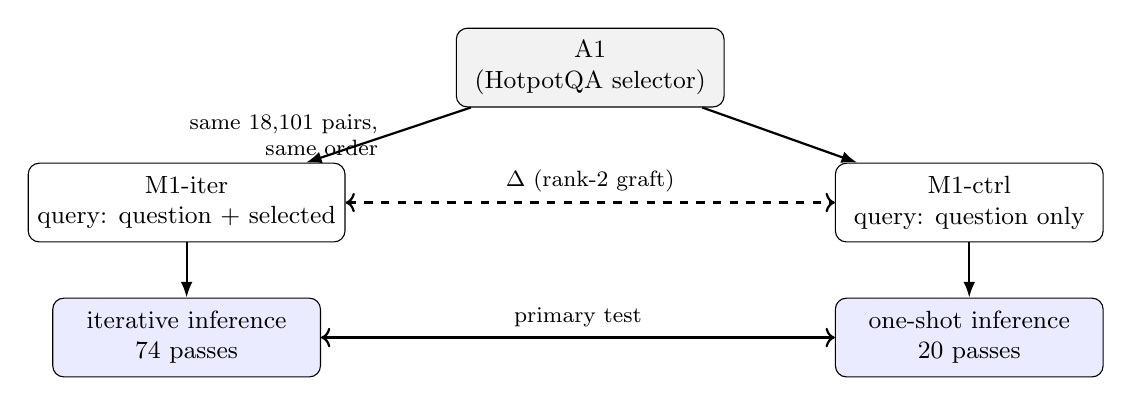
\begin{tikzpicture}[
  box/.style={draw, rounded corners, align=center, minimum width=3.4cm, minimum height=1.0cm, font=\small},
  arr/.style={-{Latex[length=2mm]}, thick},
  node distance=0.7cm and 1.4cm]
  \node[box, fill=gray!10] (a1) {A1\\(HotpotQA selector)};
  \node[box, below left=of a1] (iter) {M1-iter\\query: question + selected};
  \node[box, below right=of a1] (ctrl) {M1-ctrl\\query: question only};
  \node[box, below=of iter, fill=blue!8] (ei) {iterative inference\\74 passes};
  \node[box, below=of ctrl, fill=blue!8] (ec) {one-shot inference\\20 passes};
  \draw[arr] (a1) -- node[left, font=\footnotesize, align=right] {same 18,101 pairs,\\same order} (iter);
  \draw[arr] (a1) -- (ctrl);
  \draw[arr] (iter) -- (ei);
  \draw[arr] (ctrl) -- (ec);
  \draw[<->, thick, dashed] (iter) -- node[above, font=\footnotesize] {$\Delta$ (rank-2 graft)} (ctrl);
  \draw[<->, thick] (ei) -- node[above, font=\footnotesize] {primary test} (ec);
\end{tikzpicture}

\caption{Pair-matched control. Both models start from A1 and see the same paragraphs, labels and order; only the query differs. Each is evaluated in the inference mode it was trained for, and their weight difference $\Delta$ is analysed by grafting.}
\label{fig:matched}
\end{figure}

The pre-registered secondary test asked whether the pure conditioning change, $\Delta = \text{M1-iter} - \text{M1-ctrl}$, is also low-rank. Grafted onto M1-ctrl at rank 2, it recovered 86.8\% of the effect on the test set (CI $[77.7\%, 95.8\%]$), while a random rank-2 change of the same norm recovered 7\%. Without this change, M1-ctrl collapses when run iteratively (recall@5 of 0.41), so $\Delta$ encodes the ability to \emph{read} a conditioned query.

\section{The effect is concentrated on long chains}
\label{sec:res_long}

An exploratory reading of the matched control suggested that the gain was concentrated on four-hop questions. This was tested on 566 fresh four-hop questions (166 unused development questions and 400 unused training questions). M1-iter (iterative) beat M1-ctrl (one-shot) by 0.055 recall@5 (0.500 vs 0.445, CI $[0.007, 0.102]$, $p=0.035$), positive in both sources ($+0.139$ and $+0.020$) and for all three seeds. On all 1,017 fresh development questions (exploratory), the gain was about zero on two-hop questions, $+0.078$ on three-hop ($p=0.010$) and $+0.139$ on four-hop questions ($p=0.006$).

A cascade that runs the one-shot ranker for every question and the iterative one only for questions predicted to be four-hop did not help: it routed 29\% of questions, reached 0.702 recall@5 with 41.5 passes, against 0.693 for one-shot (20 passes) and 0.745 for always-iterative (74 passes), and failed both pre-registered tests. The router predicted hop count reasonably (four-hop recall 0.76, precision 0.43), but not the questions where iteration actually helps.

\section{Answer quality}
\label{sec:res_f1}

\todo[inline]{exp15 (running): answer F1 of gpt-5.4-mini with the top-5 sets of M1-ctrl and M1-iter on the fresh development questions; pre-registered primary on questions with three or more hops, order-controlled.}

\section{Summary}

Table~\ref{tab:claims} lists the claims and their status. The practical result is that a small in-domain selector with adaptive stopping is the cost-efficient choice. The research result is that the ability to follow an evidence chain is a separable rank-2 change in such a selector, with a measurable benefit on long chains only, and that simple routing does not yet capture that benefit.

\begin{table}[htbp]
\centering
\caption{Claims and their status (C = confirmed by a pre-registered test; N = null; E = exploratory).}
\label{tab:claims}
\small
\begin{tabularx}{\textwidth}{>{\raggedright\arraybackslash}Xll}
\toprule
Claim & Status & Section \\
\midrule
Small selector: 68--77\% fewer tokens at equal F1 (HotpotQA) & C & \ref{sec:res_selector} \\
Adaptive stopping saves tokens at a recall target & C & \ref{sec:res_adaptive} \\
Iteration beats one-shot at matched training data & N ($+0.040$, $p=0.11$) & \ref{sec:res_matched} \\
The conditioning change is rank 2 & C (86.8\%) & \ref{sec:res_rank}, \ref{sec:res_matched} \\
Iteration helps four-hop chains & C ($+0.055$) & \ref{sec:res_long} \\
Iteration helps three-hop chains, not two-hop & E & \ref{sec:res_long} \\
A hop-count router gives a useful cascade & N & \ref{sec:res_long} \\
\bottomrule
\end{tabularx}
\end{table}

\chapter{Research Plan}
\label{chap:plan}

\section{Expected contribution}

The dissertation will defend the hypothesis of Chapter~\ref{chap:intro} and deliver a reusable artifact (Figure~\ref{fig:pipeline}):
\begin{enumerate}
  \item a small one-shot selector, fine-tuned for multi-hop evidence, with adaptive stopping;
  \item a \emph{chain adapter}: a rank-2 update (about 180,000 parameters, under 1\% of the model) that turns the one-shot selector into an iterative one. A single base model then serves both modes;
  \item a router that decides, per question, whether to activate the adapter;
  \item an evaluation script that reports tokens, passes, full-support recall and answer quality against fixed top-$k$, Adaptive-$k$ and always-iterative baselines.
\end{enumerate}
The adapter saves memory and deployment complexity, not passes: activating it still costs iterative inference. Savings in passes depend on the router.

\begin{figure}[htbp]
\centering
\resizebox{\textwidth}{!}{% Planned system: cheap selector, router and rank-2 chain adapter (TikZ).
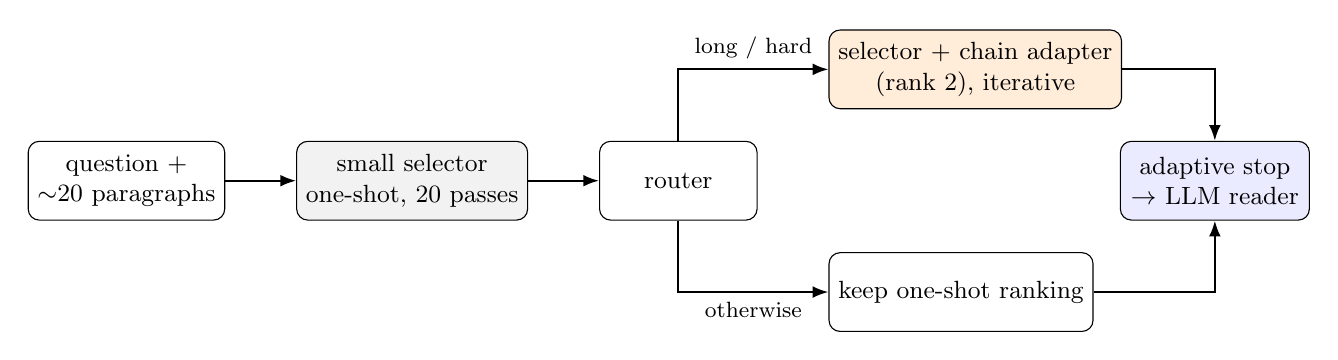
\begin{tikzpicture}[
  box/.style={draw, rounded corners, align=center, minimum height=1.0cm, font=\small},
  arr/.style={-{Latex[length=2mm]}, thick},
  node distance=0.6cm and 0.9cm]
  \node[box, minimum width=2.2cm] (q) {question +\\$\sim$20 paragraphs};
  \node[box, right=of q, fill=gray!10, minimum width=2.8cm] (sel) {small selector\\one-shot, 20 passes};
  \node[box, right=of sel, minimum width=2.0cm] (rt) {router};
  \node[box, above right=0.4cm and 0.9cm of rt, fill=orange!15, minimum width=3.2cm] (ad) {selector + chain adapter\\(rank 2), iterative};
  \node[box, below right=0.4cm and 0.9cm of rt, minimum width=3.2cm] (keep) {keep one-shot ranking};
  \node[box, right=4.6cm of rt, fill=blue!8, minimum width=2.4cm] (llm) {adaptive stop\\$\rightarrow$ LLM reader};
  \draw[arr] (q) -- (sel);
  \draw[arr] (sel) -- (rt);
  \draw[arr] (rt) |- node[pos=0.75, above, font=\footnotesize] {long / hard} (ad);
  \draw[arr] (rt) |- node[pos=0.75, below, font=\footnotesize] {otherwise} (keep);
  \draw[arr] (ad) -| (llm);
  \draw[arr] (keep) -| (llm);
\end{tikzpicture}
}
\caption{Planned system. The cheap one-shot selector runs for every question; the router activates the rank-2 chain adapter only where iteration is expected to help; adaptive stopping decides how many paragraphs reach the LLM.}
\label{fig:pipeline}
\end{figure}

\section{Remaining work}

\begin{description}
  \item[W1. Train the adapter directly.] So far the rank-2 change was extracted from a full fine-tuning run. Training a rank-1, 2 and 4 LoRA \cite{hu2022lora} on the same pairs will show whether the artifact can be built directly, and how it compares with the extracted one \cite{biderman2024loralearnsless,shuttleworth2025illusion}.
  \item[W2. Router trained on benefit.] The hop-count router failed (Section~\ref{sec:res_long}). A router trained to predict, per question, whether iteration improves the top five is pre-registered and waiting for GPU time.
  \item[W3. Answer quality.] Whether the recall gain on long chains reaches the reader's answers (Section~\ref{sec:res_f1}).
  \item[W4. Geometry with noise baselines.] Singular-value energy, stable rank and principal angles of the conditioning change, compared with seed-to-seed differences and random matrices \cite{altaf2026noisebaseline}, to separate functional rank from spectral structure.
  \item[W5. Transfer.] Graft the adapter onto other one-shot rerankers (A1, the off-the-shelf MS MARCO model) and evaluate on 2WikiMultiHopQA \cite{ho2020twowiki}. Transfer of a behaviour, not only a domain, between rerankers would be the main novelty \cite{braga2025taskarithmetic}.
\end{description}

\section{Threats to validity}

\begin{itemize}
  \item \textbf{Effect size.} The confirmed gain on long chains is modest ($+0.055$ recall@5 on four-hop questions) and heterogeneous between data sources.
  \item \textbf{Single architecture and data source.} All selectors are MiniLM-L6 and all evaluation questions come from MuSiQue (and HotpotQA for the first results). W5 addresses this.
  \item \textbf{Evaluation sets.} MuSiQue test labels are not public; evaluation uses disjoint subsets of the development split, and one fresh set has been used twice (with the second use declared in advance).
  \item \textbf{Multiplicity.} Each experiment has a single primary test; across experiments no correction is applied. The headline claims will be re-tested on a locked set before the defence.
\end{itemize}

\section{Schedule}

Table~\ref{tab:schedule} lists the planned activities by quarter.

\begin{table}[htbp]
\centering
\caption{Schedule (quarters from the qualification).}
\label{tab:schedule}
\small
\begin{tabular}{lcccc}
\toprule
Activity & Q1 & Q2 & Q3 & Q4 \\
\midrule
W1 adapter trained directly; W3 answer quality & $\bullet$ & & & \\
W2 benefit router and cascade & $\bullet$ & $\bullet$ & & \\
W4 geometry with noise baselines & & $\bullet$ & & \\
W5 transfer across rerankers and to 2WikiMultiHopQA & & $\bullet$ & $\bullet$ & \\
Paper submission & & & $\bullet$ & \\
Locked-set confirmation of the headline claims & & & $\bullet$ & \\
Dissertation writing and defence & & & $\bullet$ & $\bullet$ \\
\bottomrule
\end{tabular}
\end{table}


\bibliography{bibli}

\appendix
\chapter{Experiment Index}
\label{app:index}

All experiments are in the project repository, each with a pre-registered protocol and a results report. Experiments not used in the main text are kept for later work.

\begin{table}[htbp]
\centering
\small
\begin{tabularx}{\textwidth}{l>{\raggedright\arraybackslash}Xl}
\toprule
ID & Question and outcome & In text \\
\midrule
exp01 & Training-free second-hop threshold on embeddings: 6--10\% fewer tokens than Noise-Gate & no \\
exp02 & Fine-tuned 22.7M selector: 68--77\% fewer tokens at equal F1 & \ref{sec:res_selector} \\
exp03 & Linear probe for multi-hop relevance in A0: probe failed (not evidence of absence) & no \\
exp04 & LLM agents editing the selector's weights: compression ties magnitude pruning; no repair & no \\
exp05 & Failure analysis: missed paragraphs are bridge paragraphs that do not name the question's entity & no \\
exp06 & A1 $-$ A0 is low-rank (rank 4: 80\%) and mid-layer; sparse grafts fail & \ref{sec:res_rank} \\
exp07 & Adaptive stopping on HotpotQA: $-57$ / $-71$ tokens & \ref{sec:res_adaptive} \\
exp08 & A1 on MuSiQue: top-10 recall 0.68; planned comparison not testable & \ref{sec:res_bottleneck} \\
exp09 & In-domain and iterative fine-tuning: recall@5 0.682 / 0.750 (confounded) & \ref{sec:res_bottleneck} \\
exp10 & Adaptive stopping on the iterative ranker; Adaptive-$k$ addendum & \ref{sec:res_adaptive} \\
exp11 & The iteration change is rank 2 (84.7\%) & \ref{sec:res_rank} \\
exp12 & Pair-matched control: $+0.040$ (n.s.); conditioning change rank 2 (86.8\%) & \ref{sec:res_matched} \\
exp13 & Fresh four-hop confirmation ($+0.055$); hop-count cascade fails & \ref{sec:res_long} \\
exp14 & Router trained on benefit: $+0.027$ vs one-shot with 41 of 74 passes & \ref{sec:res_long} \\
exp15 & Answer F1 on $\ge$3-hop questions: $+0.076$; top 5 beats all paragraphs & \ref{sec:res_f1} \\
exp16 & Rank-2 replication: 97.1\% (2WikiMultiHopQA), 92.1\% (HotpotQA) & \ref{sec:res_replication} \\
\bottomrule
\end{tabularx}
\end{table}


\end{document}
